\documentclass[]{acm_proc_article-sp}

% from Pandoc standard LaTeX templates
\usepackage[T1]{fontenc}
\usepackage{lmodern}
\usepackage{amssymb,amsmath}
\usepackage{ifxetex,ifluatex}
\usepackage{fancyvrb,relsize}
\usepackage{parskip}
\usepackage{fixltx2e} % provides \textsubscript
% use upquote if available, for straight quotes in verbatim environments
\IfFileExists{upquote.sty}{\usepackage{upquote}}{}
\ifnum 0\ifxetex 1\fi\ifluatex 1\fi=0 % if pdftex
  \usepackage[utf8]{inputenc}
\else % if luatex or xelatex
  \usepackage{fontspec}
  \ifxetex
    \usepackage{xltxtra,xunicode}
  \fi
  \defaultfontfeatures{Mapping=tex-text,Scale=MatchLowercase}
  \newcommand{\euro}{€}
\fi
% use microtype if available
\IfFileExists{microtype.sty}{\usepackage{microtype}}{}
\ifxetex
  \usepackage[setpagesize=false, % page size defined by xetex
              unicode=false, % unicode breaks when used with xetex
              xetex]{hyperref}
\else
  \usepackage[unicode=true]{hyperref}
\fi
\urlstyle{same}  % don't use monospace font for urls
\setlength{\parindent}{0pt}
\setlength{\parskip}{6pt plus 2pt minus 1pt}
\setlength{\emergencystretch}{3em}  % prevent overfull lines
\setcounter{secnumdepth}{0}

\DefineVerbatimEnvironment{verbatim}{Verbatim}{frame=single,framerule=0.5pt,framesep=0.4em,numbers=none,numbersep=0.5em,stepnumber=1,numberblanklines=true,fontsize=\relsize{-3}}

\pagenumbering{arabic}

\begin{document}

\title{P x B + D \textgreater{} C: a ``calculus'' for Open Data}



\author{
  %\alignauthor 
  Arnaud Sahuguet
      \\
          \affaddr{The Governance Lab at NYU}\\
          \affaddr{Brooklyn, New York, USA}\\
        \email{arnaud.sahuguet@gmail.com}
  \and
  %\alignauthor 
  David Sangokoya
      \\
          \affaddr{The Governance Lab at NYU}\\
          \affaddr{Brooklyn, New York, USA}\\
        \email{david.sangokoya@gmail.com}
  \and
}

\conferenceinfo{Data4Good Exchange}{Bloomberg's Data for Good Exchange 2015}
\copyrightetc{CC-Zero  Arnaud Sahuguet  David Sangokoya  28 Sep 2015}



\date{2015-08-14}

\maketitle

\begin{abstract}
Open data makes great promises and offers untapped benefits for
individual, public and private decision-making. However, these benefits
often come with hidden costs and risks to data providers. In deciding
whether or not to open up their data, decision makers - across all
sectors and at all levels - often do not fully understand the levers
they can operate or in which direction to pull them. Taking some
inspiration from ``A theory of the calculus of voting'' {[}12{]}, we
present a modest attempt at formalizing a ``calculus of open data'' to
help data providers make this decision.
\end{abstract}

%%
%%
%%

\section{Introduction}\label{introduction}

The value, impact and promise of making data publicly accessible have
driven citizens, government agencies and businesses to embrace open data
as a way to increase efficiency, promote transparency and maximize
utility.

``Open data is data that can be freely used, reused and redistributed by
anyone - subject only, at most, to the requirement to attribute and
share-alike'' {[}1{]}. McKinsey {[}8{]} estimates more than \$3 trillion
in additional value globally as a result of open data. Large scale
studies such as the Open Data 500 reveal an impact across sectors such
as energy, consumer products and healthcare. More than 40 countries have
shared over a million government datasets. Shared corporate data
provides mutual benefits for both public and private sector entities,
e.g.~Uber's partnership with the City of Boston {[}19{]}, the
Twitter-MIT Laboratory for Social Machines {[}9{]}and Yelp's Dataset
Challenge {[}22{]}.

While the rise of the open data movement has led to numerous commitments
and increasing enthusiasm to unleash the potential of open data, data
providers lack a common language for evaluating and weighing the
decision to open their own data.

Government agencies and city officials often open their data as a result
of top-down pressure to champion efficiency, meet citizen demand or
increase transparency through the number of datasets released rather
than the impact these datasets may create. They often do not understand
the hidden costs associated with opening their data and miss
opportunities to leverage knowledge from communities or outside
expertise for optimal data sharing.

Corporations are mostly embracing a wait-and-see attitude. While some
have begun sharing corporate data for research or policymaking intended
for public benefit, others are building business models from public open
data. Since data is seen as a business asset holding significant value,
companies are cautiously considering why they should take on risks to
competition and engage in activity amidst nascent legal and regulatory
frameworks.

End users are motivated to share their data. However, they often are not
the true \textbf{owners}, their data being stored and managed on their
behalf by technology and social media companies. Even when they are, the
fear of unwanted government surveillance or corporate marketing
practices dissuades them from making their data more publicly
accessible.

\section{Stories from the field}\label{stories-from-the-field}

We briefly start with a few selected examples to highlight the value and
impact of open data and the need for a better decision framework when
choosing to open data.

\subsection{Success and horror
stories}\label{success-and-horror-stories}

We've seen the success stories and numerous examples of open data.
Public transit information (made available by cities via Google GTFS
standard) is saving time to millions of people on a daily basis. GPS
data is at the core of mobile location-based services and products.
Weather information from the National Oceanic and Atmospheric
Administration (NOAA) is used by weather companies and insurance agents
such as The Weather Channel and the Climate Corporation. The open nature
of the data in the Human Genome Project fostered at-scale collaboration
in decoding the genome and creating an ecosystem of innovation among
academic and private researchers.

We've also witnessed the horror stories. A seminal example was the
release of search logs by AOL for academic research purposes in 2006.
The released data contained some publicly-identifiable information (PII)
on AOL members that made it possible to identify people and reveal their
internet search histories. More recently, the release of improperly
anonymized taxi data from the New York City Taxi \& Limo Commission
revealed the identities of taxi drivers, trips of celebrities and even
the religious orientation of some drivers.

\subsection{The hard questions}\label{the-hard-questions}

For all these cases, here are some questions that are hard to answer
today:

\vspace{0mm}

\begin{enumerate}
\itemsep1pt\parskip0pt\parsep0pt
\item
  why did stakeholders choose to open (or not open) their data?
\item
  what incentives could have been put in place to encourage (or
  discourage) opening and sharing of data?
\item
  among the various levers one can pull, which one makes the most sense
  for the data provider?
\end{enumerate}

\section{A calculus for open data}\label{a-calculus-for-open-data}

Our calculus centers around a simple equation:

\begin{equation}
P \times B + D > C
\end{equation}

where

P is the probability that opening the data will have some effect, B is
the individual benefit of opening the data, D is the global or ecosystem
impact, and C is the cost. Any increase in P, B or D and a decrease in C
will make the outcome of opening the data better.

Let's now revisit each variable one by one and look at concrete factors
that influence it.

\subsection{P for probability}\label{p-for-probability}

\emph{P} represents the probability that opening the data will generate
potential benefits for the data owner.

Factors that make \emph{P} go up include: \vspace{0mm}

\begin{itemize}
\itemsep1pt\parskip0pt\parsep0pt
\item
  standards to publish the data
\item
  a data-driven culture inside public and private sectors, fostered by
  strong education offerings.
\item
  an ecosystem of data consumers, with a hackers/developers to build
  products, clearinghouses to store and curate data (e.g.~Enigma), data
  science shops (e.g.~Kaggle, DataKind, Bayes Impact).
\item
  incentives for consumers to use the data, e.g.~prizes \& challenges
  (NYC BigApps, Netflix Prize) or funded research (e.g.~Twitter Data
  Grants).
\end{itemize}

Factors that make \emph{P} go down include: \vspace{0mm}

\begin{itemize}
\itemsep1pt\parskip0pt\parsep0pt
\item
  the absence or inflexibility of legal frameworks, e.g.~rigid or
  non-existent legal framework around data
\item
  the lack of trust among the various players.
\end{itemize}

\subsection{B for benefits}\label{b-for-benefits}

The potential benefits \emph{B} for the entity opening data include
benefits about the quality improvement for the data after being
released: \vspace{0mm}

\begin{itemize}
\itemsep1pt\parskip0pt\parsep0pt
\item
  better accuracy and less errors as a result of public scrutinization
  of the data less gaps in the data in terms of coverage \& granularity
  coming from external contribution
\item
  better interoperability as a result of un-siloed data sustainability
  of data
\item
  data prioritization, to help identity most impactful datasets
\item
  improved data collection by other public institutions (decreasing
  unnecessary duplication and associated costs)
\end{itemize}

Interesting findings about the data may be valuable and result in
increased political, social and economic benefits for the data owner,
including: \vspace{0mm}

\begin{itemize}
\itemsep1pt\parskip0pt\parsep0pt
\item
  development of new products and services
\item
  creation of new insights in the public sector
\item
  creation of a new sector adding value to the economy
\item
  creation of new data based on combining data
\item
  visibility and publicity for the data provider
\item
  improvement of citizen services
\end{itemize}

This category of benefits varies greatly based on the type of data being
opened up.

In addition, opening the data might create some monetization
opportunities. For instance, a city could sell access to real-time feeds
of its data (e.g.~to hedge funds, insurance companies) while making the
exact same data publicly accessible but delayed on its portal within a
week.

\subsection{D for duty}\label{d-for-duty}

\emph{D} stands for Duty in the original paper. In our setting it
translates more into ``ecosystem impact'' or ``global impact'', and is
industry specific. This represents the positive impact of opening the
data for other players.

Public entities will see the value of opening the data in terms of
better governance (transparency, democratic accountability,
collaboration, participation), improved quality-of-life for citizens,
better government-to-government interactions, equal access to data and
better economic development.

Private entities will see the value more in terms of corporate social
responsibility.

End users will see value in terms of social responsibility and
pro-social behavior.

\subsection{C for costs}\label{c-for-costs}

Finally \emph{C} stands for cost which is influenced by the following
factors. \vspace{0mm}

\begin{itemize}
\item
  Opening costs, i.e.~the costs of opening the data itself. These costs
  involve the costs of transitioning data buried inside legacy systems
  and reformatting the data into an open format.
\item
  Operating costs, i.e.~the cost of publishing the data and keeping it
  fresh. Even with affordable commercial offerings and open source
  solutions, there is still a cost in running an open data portal.
\item
  Quality costs, i.e.~costs of keeping the data fresh.
\item
  Legal costs, i.e.~costs of opening the data in compliance with the
  various legislations. Finding legal expertise in this relatively new
  field can be hard to find and therefore expensive; this is even worse
  when dealing with multiple legal jurisdictions lacking harmonization
  (e.g.~Europe vs.~U.S.).
\item
  Liability costs and risks, i.e.~the costs when something goes wrong
  such as privacy, erroneous data, stale data. Again, the lack of legal
  clarity makes this risk harder to quantify.
\item
  Mandatory costs, i.e.~when opening the data is a legal requirement
  (resp. a right) and not doing so results in fines (resp. cost,
  e.g.~FOIA in the U.S.).
\item
  Competitive cost (for corporations), i.e.~the cost of sharing
  information that can be used by the competition.
\item
  Privacy cost (for individuals), i.e.~the cost of sharing information
  that can be used to reduce quality of life, e.g.~spam, insurance
  premium, etc.
\item
  Public relations costs, i.e.~the cost incurred from bad press due to
  information gleaned from the data, e.g.~performance metrics for a
  city, environment metrics or workforce diversity for a corporation.
\item
  Opportunity costs, because the same resources (money, technical
  infrastructure, human resources) could be spent doing something else.
\item
  Particular categories of costs (e.g.~transition, privacy, opportunity)
  will vary based on each industry.
\end{itemize}

\begin{figure*}[htbp]
\centering
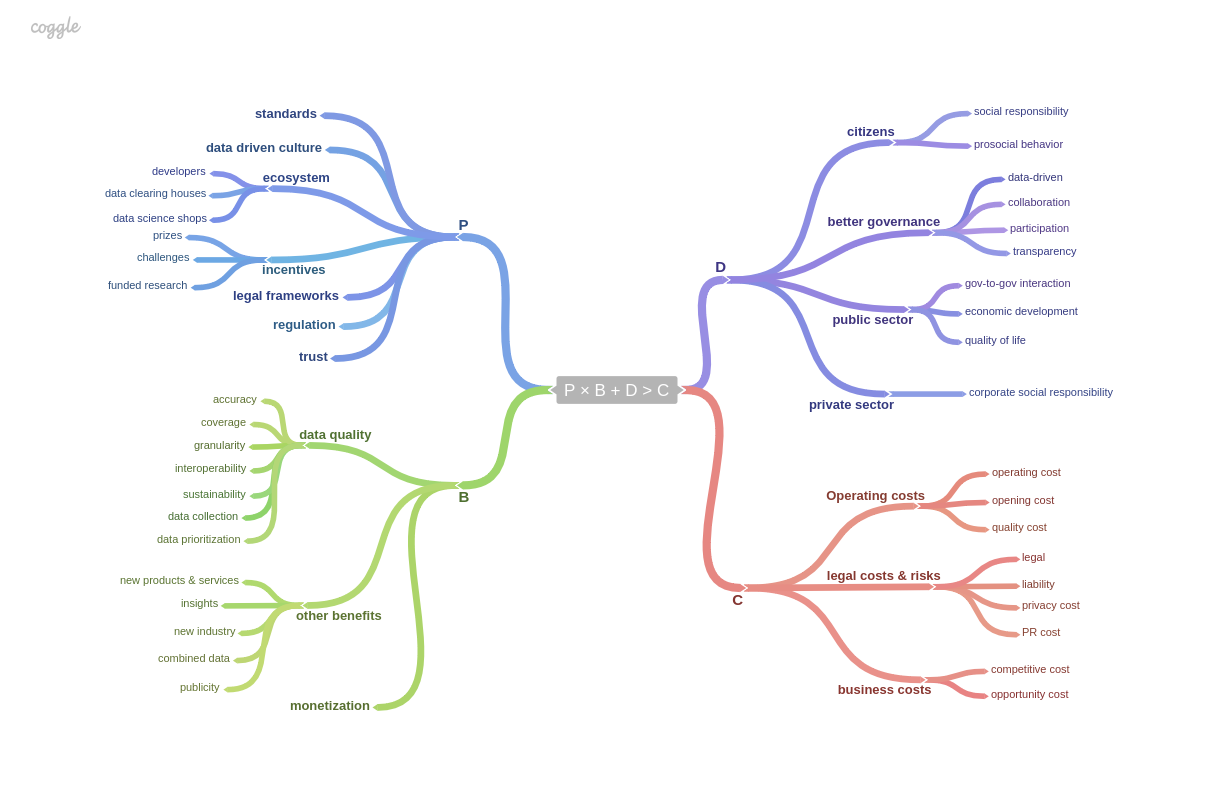
\includegraphics[width=\textwidth]{images/pbdc_equation.png}
\caption{The various factors}
\end{figure*}

\subsection{Pulling the levers}\label{pulling-the-levers}

The equation describes a quantity that should be greater than zero for
opening the data to make sense. In some practical situations, some
variables may be beyond the control of the data owner. The equation
provides guidance in terms of what levers can be used and points to
additional decisions to be considered.

\textbf{Focus on P: increase probability of benefits} \vspace{0mm}

\begin{itemize}
\itemsep1pt\parskip0pt\parsep0pt
\item
  Have we invested in the right people, culture to move this initiative
  forward?
\item
  How usable is the data for a hacker community to build off of? Focus
  on B: increase benefits from the data
\item
  Is there an easy mechanism for users of the data to provide some
  feedback?
\item
  How does the data interact with related datasets and systems
  (e.g.~interoperability)?
\end{itemize}

\textbf{Focus on D: value duty and ecosystem impact} \vspace{0mm}

\begin{itemize}
\itemsep1pt\parskip0pt\parsep0pt
\item
  What's the potential value chain impact from opening up the data? Who
  benefits from opening up this data?
\item
  What relationships or goodwill can we forge by making this decision?
\end{itemize}

\textbf{Focus on C: reduce costs} \vspace{0mm}

\begin{itemize}
\itemsep1pt\parskip0pt\parsep0pt
\item
  What are the real costs in transitioning and reformatting data into a
  usable format?
\item
  What are the maintenance costs associated with opening the data?
\end{itemize}

The nature of the equation involves weighing a combination of approaches
increasing P, B and D while decreasing C. The following examples
illustrate these approaches in action toward more optimal sharing.

\section{Revisiting 3 examples}\label{revisiting-3-examples}

We revisit 3 typical use cases for open data and see how the calculus
can help identify the levers that can be used to improve the outcome.

\subsection{Example 1: API}\label{example-1-api}

Cities (and governments more generally) often start their open data
efforts by simply offering raw access to their bulk datasets and only
consider API as an after thought. That's often an oversight.

APIs force the use of standards (P\(\uparrow\)); facilitate the
organization of prize and challenges (P\(\uparrow\)).

APIs are by nature hacker-friendly (P\(\uparrow\)). APIs are also the
natural conduit for data monetization (P\(\uparrow\)).

APIs can be expensive to create and maintain (C\(\uparrow\)); but they
also provide a better data granularity which helps with privacy and can
reduce legal liabilities (C\(\downarrow\)).

So overall, APIs usually look like a good value proposition. Access to
affordable tools and pre-existing standards can reduce the cost even
more and make this option a no-brainer.

\subsection{Example 2: City Data
Portals}\label{example-2-city-data-portals}

The city data portal is the web presence where a city decides to publish
the datasets it is opening.

First, running such a portal costs money in terms of storage and
bandwidth (C\(\uparrow\)) . If the portal permits to run complicated
queries against the data, a computation cost gets introduced
(C\(\uparrow\)). If the portal contains some social features like a
forum, a community manager is needed (C\(\uparrow\)) to handle people's
request and handle communication issues.

A good data portal will make the data easier to discover for end users
(P\(\uparrow\)).

User feedback will improve the quality of the data (B\(\uparrow\)) and
increase user engagement (P\(\uparrow\), D\(\uparrow\)).

A good data portal will also benefit city agencies who can discover and
leverage each other's data (D\(\uparrow\)). Proactively opening the data
is also a good way to avoid numerous and expensive FOIA requests
(C\(\downarrow\)).

Given the availability of good data portal tools (e.g.~Socrata, CKAN,
Github) and cheap hosting, the cost C is often low and a City Data
Portal is usually a good option.

\subsection{Example 3: Citizen Digital
Philanthropy}\label{example-3-citizen-digital-philanthropy}

User data can be very useful for research purposes for instance in the
medical field or urban planning field. As a civic minded user, I am
interested in donating my personal data. P, B and D are already high.
But so is C.

In most cases, my data is actually locked at/by some provider which
makes it hard to share in the first place (C\(\uparrow\)). Also, there
is little guarantee about the respect of my privacy (C\(\uparrow\)).
There is also a risk that the data I open will not be used for the exact
purpose I have in mind which is captured in our equations by a lower
benefit (B\(\downarrow\)).

In this use case, the critical element seems to be cost. The existence
of data clearinghouses that can anonymize data and guarantee the
appropriate use of the data (per the user's request) would make such
form of philanthropy possible to user by reducing C. The use case also
requires an environment where the user is actually in control of her
data.

\section{Conclusion}\label{conclusion}

A simple equation will not answer all the questions about open data.
Despite all its limitations, we think that this ``calculus'' can be
useful as a way of anchoring the conversation, similar to Anthea Watson
Strong's The Three Levers of Civic Engagement {[}16{]}.

Looking at the formula, decision makers can see how a given factor
influences the outcome. Internally, the formulation could form the logic
basis for a performance measurement and decision making tool.
Externally, this could be extremely valuable for governments trying to
engage the private sector in sharing private sector data or for the tech
community in identifying technologies that would reduce cost or amplify
benefits.

By just looking at the levers, one can reasonably anticipate that (1)
data marketplaces where corporations can exchange data, (2) trusted 3rd
parties offering aggregation and anonymization of end user data and (3)
templates --- both legal and database schemas --- incorporated in
software portal solutions would make decisions to open data more
feasible and rational for data providers.

We hope that our ``calculus'' for open data can better frame the
question of opening the data, help identify the various levers that can
be pulled and facilitate conversations and research on this topic at all
levels.

\section*{References}\label{references}
\addcontentsline{toc}{section}{References}

{[}1{]} Dietrich, D. et al. 2009. Open data handbook.
\href{http://opendatahandbook. org}{http://opendatahandbook. org}.

{[}2{]} Eckartz, S.M. et al. 2014. A decision model for data sharing.
\emph{Electronic government}. Springer Berlin Heidelberg. 253--264.

{[}3{]} Grabar, H. 2015. Would you share private data for the good of
city planning? Next City.

{[}4{]} Gurin, J. 2014. \emph{Open data now}. McGraw Hill Education.

{[}5{]} Howard, A. 2014. More than economics: The social impact of open
data. \emph{Tech Republic}. (31\textasciitilde{}jul 2014).

{[}6{]} Janssen, M. et al. 2012. Benefits, adoption barriers and myths
of open data and open government. \emph{Information Systems Management}.
29, 4 (2012), 258--268.

{[}7{]} Kirkpatrick, R. 2011. Data philanthropy: Public \& private
sector data sharing for global resilience. \emph{UN Global Pulse}. 16,
(2011).

{[}8{]} Manyika, J. 2013. \emph{Open data: Unlocking innovation and
performance with liquid information}. McKinsey.

{[}9{]} MIT Media Lab Laboratory for social machines.
\url{http://socialmachines.media.mit.edu/}.

{[}10{]} Pawelke, A. and Tatevossian, A.R. 2013. Data philanthropy:
Where are we now. \emph{United Nations Global Pulse Blog}. (2013).

{[}11{]} Penner, L.A. et al. 2005. Prosocial behavior: Multilevel
perspectives. \emph{Annu. Rev. Psychol.} 56, (2005), 365--392.

{[}12{]} Riker, W.H. and Ordeshook, P.C. 1968. A theory of the calculus
of voting. \emph{Am. Polit. Sci. Rev.} 62, 01 (1968), 25--42.

{[}13{]} Sahuguet, A. et al. 2014. Open civic data: Of the people, by
the people, for the people. \emph{Data Engineering Bulletin}. (Dec.
2014).

{[}14{]} Skatova, A. and Goulding, J. 2015. Donated personal data could
aid lifestyle researchers. Scientific American.

{[}15{]} Skatova, A. et al. Data donation: Sharing personal data for
public good?

{[}16{]} Strong, A.W. 2014. The three levers of civic engagement.
\emph{Medium}.
\url{https://medium.com/thelist/the-three-levers-of-civic-engagement-cde106b68523}.

{[}17{]} Sunlight Foundation 2014. \emph{The impacts of open data}.
Sunlight Foundation.

{[}18{]} Tauberer, J. 2012. \emph{Open government data}.

{[}19{]} Uber 2015. Driving solutions to build smarter cities.
\url{http://newsroom.uber.com/boston/2015/01/driving-solutions-to-build-smarter-cities/}.

{[}20{]} Verhulst, S. 2014. \emph{Mapping the next frontier of open
data: Corporate data sharing}. UN Global Pulse.

{[}21{]} Wellington, B. I quant NY. \emph{I quant NY}.
\url{http://iquantny.tumblr.com/}.

{[}22{]} Yelp Yelp dataset challenge.
\url{http://www.yelp.com/dataset_challenge}.

{[}23{]} Zuiderwijk, A. et al. 2014. Special issue on innovation through
open data: Guest editors' introduction. \emph{Journal of theoretical and
applied electronic commerce research}. 9, 2 (2014), i--xiii.

\end{document}
